\documentclass[10pt,letterpaper]{article}
\usepackage{geometry}
\geometry{margin=1in}
\usepackage{graphicx}
\usepackage{svg}
\usepackage{float}

\setlength{\parindent}{0pt}
\setlength{\parskip}{0.5em}

%make lists tighter
\usepackage{enumitem}
\setlist{nolistsep}

%reduce spacing before and after section
\usepackage{titlesec}
\titlespacing\section{0pt}{6pt}{0pt}

\title{Lab 1 - PECARN TBI Data, STAT 214, Spring 2025}

% submission must not contain your name
% but feel free to make a version for yourself with your name on it
\author{}

\begin{document}
\maketitle

\section{Introduction}\label{introduction}

Pediatric traumatic brain injury (TBI) is a critical challenge in emergency medicine with potential long-term cognitive, neurological, and developmental consequences. Rapid and accurate assessment is essential to determine the need for computed tomography (CT) scanning. However, weighing the risks is complex: while excessive CT scans expose children to radiation and increase lifetime risk of malignancy, failure to detect a clinically significant TBI (ciTBI) can lead to serious complications or death. This highlights the need for data-driven clinical decision support systems to improve risk assessment and reduce unnecessary imaging.

This report examines the Pediatric Emergency Care Applied Research Network TBI dataset, detailing data collection methods, preprocessing steps, and strategies for dealing with missing values, inconsistencies, and outliers. We then conduct exploratory data analysis to uncover patterns in the data and identify different phenomena in the data. Finally, we implement a random forest model and a neural network, leveraging their interpretability and predictive power to identify children at risk for clinically significant TBI. Our findings are expected to contribute to precision medicine approaches, optimize CT scan utilization, and improve clinical decision making in pediatric emergency care.

\section{Data}\label{data}

The dataset is from a PECARN cohort study of children under 18 years of age with mild head trauma, with the aim of developing clinical prediction rules to identify low-risk cases for which CT scans can be avoided.

The data includes patient history, mechanism of injury, symptoms, clinical signs, and CT results, recorded before imaging results were known. Key variables include mechanism of injury, loss of consciousness, neurological deficits, seizures, and CT findings such as intracranial hemorrhage, contusions, and skull fractures. Follow-up data tracks missed TBIs through hospital records and physician quality assurance reviews.

This data is critical to optimizing the use of CT scans in pediatric emergency care, enabling data-driven risk assessment that helps reduce unnecessary radiation exposure while ensuring that high-risk patients receive timely treatment. Analysis of these patterns supports better clinical decision-making and improved patient outcomes.

\subsection{Data Collection}\label{data-collection}

Data were generated through direct physician assessment in the emergency department, where trained investigators recorded clinical signs, symptoms, and injury mechanisms before imaging results were known. Follow-up data were collected through hospital records, guardian interviews, and process improvement reviews to track missed TBIs.

Most of the data is collected categorically, which means that there are often only the variants 0 (No), 1 (Yes) and Unknown (90, 91, 92). If, for example, headache was answered with Yes in the data collection, there were further subcategories that describe this symptom or the findings on CT more precisely. Only a few variables such as age are available in non-categorical form.

\subsection{Data Cleaning}\label{data-cleaning}

In this chapter, we examine the data cleaning process required to prepare this complex clinical dataset for analysis. The raw data present three main challenges: missing values (including specially coded missingness), potential outliers in clinical measures, and internal inconsistencies between related variables. Our cleaning decisions aim to strike a balance between maintaining data integrity and ensuring usefulness for downstream analysis and prediction.

\subsubsection{Outlier}
Outlier detection is an integral part of any data preprocessing to exclude extreme data points and thus obtain a consistent data set. This task presents unique challenges in our dataset because outlier detection works particularly well with continuous variables, but much less well with the categorical variables that predominate in our clinical data.

We have identified two different types of potential outliers in this dataset. First, there are values that do not belong to any of the predefined categories and therefore should not occur at all. Using the data documentation as a reference, we systematically checked each variable against its allowed values. With the exception of NA values, all entries matched their documented categorical definitions, suggesting good basic data quality control during collection. Second, we looked for unusual patterns within the valid categorical values themselves. Classical statistical outlier detection methods flagged numerous observations across different columns as potential outliers. However, closer inspection revealed that these were often clinically significant rare events rather than errors.

This analysis revealed a key challenge in clinical data preprocessing: statistically rare values often represent the most clinically important cases. While these values may pose challenges in the final modeling phase due to limited training examples, they cannot be treated as traditional outliers that should be cleaned or removed. Instead, their rarity should be specifically considered during model development, especially given the critical importance of correctly identifying severe TBI cases.

Furthermore, this conservative approach to outlier handling is consistent with the study's primary goal of developing reliable clinical decision rules. Removing rare but valid clinical presentations could potentially compromise the model's ability to identify high-risk cases requiring CT scans.

\subsubsection{Missing Data}
This subsection looks at the topic of missing values, which is covered by two different types in this data set. On the one hand, there are real missing values, which are present as NA in the data set and must be eliminated. On the other hand, the data set also contains many data points with the values 90, 91, 92, which are entered if a value could not be determined (e.g., headache assessment in babies) or the value was not recorded.

This phenomenon can be seen in the heat map in figure~\ref{fig:missing_data}. The left-hand side of the heat map shows how often values with NA are present in the data set. Apart from a few exceptional columns, this is very manageable. If, on the other hand, we also consider the values 90, 91, 92 as missing values, as shown in the heatmap on the right, a different picture emerges. It can be seen that the phenomenon of data points with the values 90, 91, 92 occurs frequently throughout the dataset.

\begin{figure}[H]
    \centering
    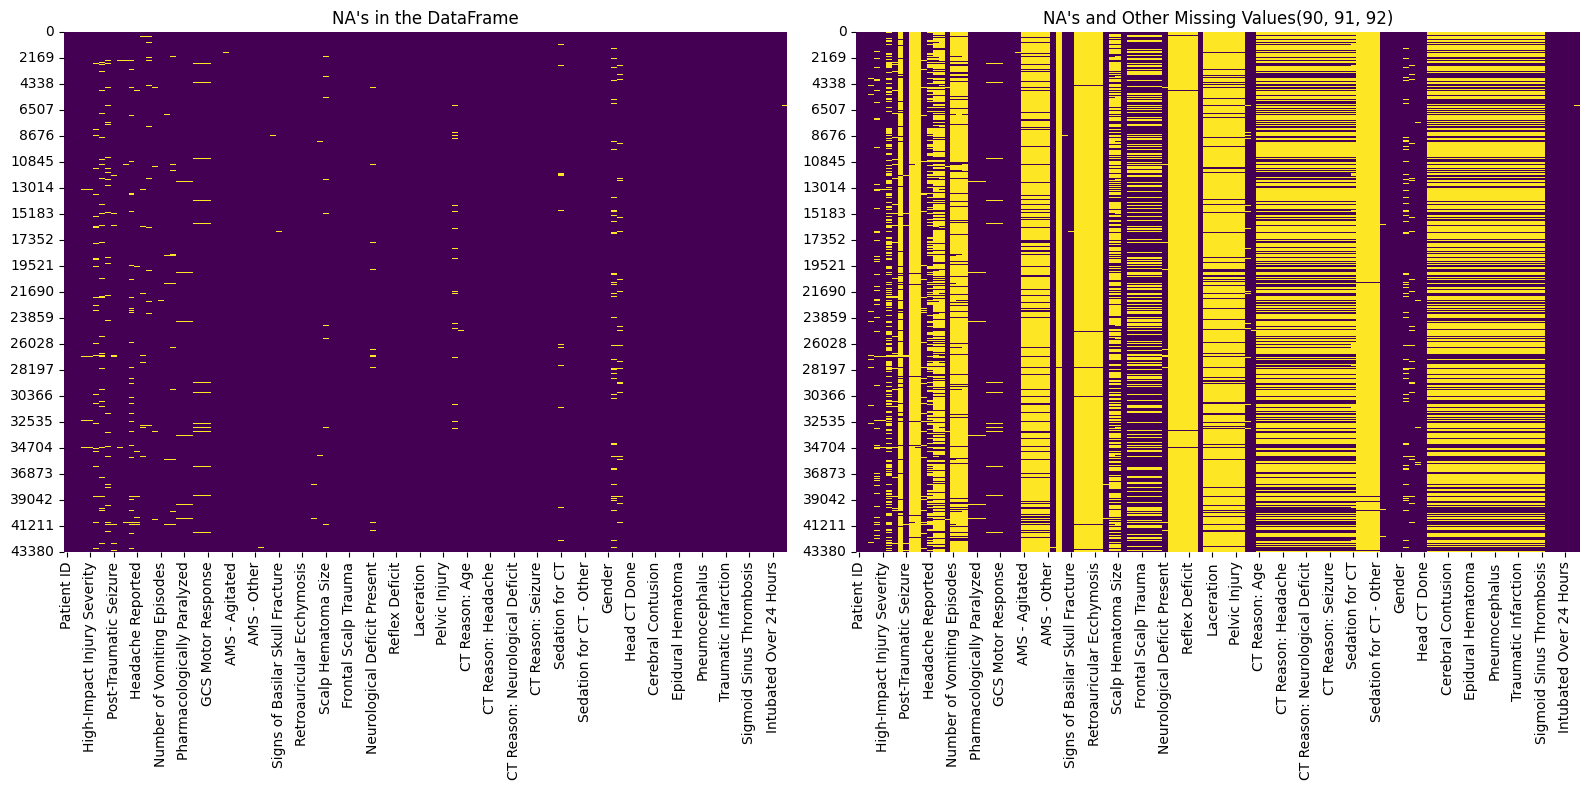
\includegraphics[width=0.8\textwidth]{../figs/missing_values.png} % Adjust width as needed
    \caption{Missing Data in the Dataset}
    \label{fig:missing_data}
\end{figure}

In the data preprocessing process, we must decide how to handle the values 90, 91 and 92. We have decided to retain these values, as they represent meaningful clinical information that would occur again in future real-world cases. For example, certain symptoms like headache cannot be assessed in very young children, making "not applicable" (91) a clinically relevant designation rather than a data quality issue.

For the NA values, we implemented the following approach:
\begin{itemize}
\item Applied logical rules where possible (e.g., calculating missing GCS component scores when total GCS is 15) to replace NAs with logical values
\item For summary variables over categories such as Scalp Hematoma Present, NAs were replaced with 0 if all dependent scores were 92 and with 1 if dependent scores were positive
\item Missing values in dependent variables were filled with 92
\item Missing values in independent variables were filled with 90/91/92 or a default value 
\item Dropped the Dizziness and Ethnicity columns which had over 30\% missing data and limited predictive value
\item Removed few rows with NA values in the critical outcome variable (e.g. ciTBI and Neurosurgery)
\end{itemize}

This processing aims to produce a dataset that maintains clinical accuracy while allowing for robust statistical analysis. The high frequency of coded missing values (90, 91, 92) reflects real-world clinical assessment challenges rather than data collection problems.

\subsubsection{Errors/Inconsistencies}

During the error or inconsistency analysis, the existing values were examined for inconsistencies that, according to the documentation, should not normally occur in the data set. This is the case, for example, if the different GCS values do not add up to the GCS total, but to a different value.

Therefore, in order to perform such an error analysis, a set of logical links was determined on the basis of the documentation in order to identify corresponding inconsistencies in the data set. Similar logical conclusions were drawn as for the missing data, so some of the considerations could be transferred from there. 

As a result of this analysis, we obtained the following graph, which identified the following problems in the corresponding categories (e.g. the four variables of GCS):

\begin{figure}[H]
    \centering
    \includesvg[width=0.8\textwidth]{../figs/inconsistencies.svg} % Adjust width as needed
    \caption{Categories for Inconsistencies before and after cleaning of Missing Data}
    \label{fig:incsonsistencies}
\end{figure}

Figure~\ref{fig:incsonsistencies} shows two pie charts comparing the distribution of inconsistencies before and after our cleaning of NA values. The left chart represents the original dataset, while the right chart shows the same analysis after applying our NA cleaning procedures. We can observe that the proportions of inconsistencies remain relatively stable across most categories, suggesting that our NA cleaning approach did not introduce new systematic inconsistencies into the data.

It is important to note that only variables that can be checked by another variable can be used here. For example, the Intubated column is not directly related to another variable, so an incorrect value in this column cannot really be determined. However, it is not so easy to correct other errors that have been identified in the error analysis. For example, in the Mental Status Issues column, we see that in some cases a status has been set, but no details about the status have been provided, and none of the subcategories have been set, although at least one category (the "Other" category exists) should be set.

Therefore, no direct error handling can be derived from this finding and it was decided to keep the rows due to the nevertheless deep information content. However, this fact that such inconsistencies are present in the data set must be taken into account in future analyses and handled if necessary.

\subsubsection{Summary Data Cleaning}

In the summary of both subchapters, the data preprocessing consists of eliminating the NA values using a sophisticated logic, eliminating the columns Dizziness and Ethnicity and the rows with NAs in ciTBI, resulting in a data set that contains all fields, but still contains the statuses 90, 91, 92, which also represents a type of unknown.

In the chapter Outlier and the Errors/Inconsistencies, mainly deeper insights were gained about the data, but after deep analysis it was decided not to derive any direct consequences from this, as otherwise the data set would become significantly smaller. Despite these identified challenges in the data, we concluded that meaningful analysis can proceed if these known issues are kept in mind during subsequent modeling and interpretation phases.

\subsection{Data Exploration}\label{data-exploration}

This chapter provides a few insights into the dataset itself, which should provide further insight into the data after data cleaning. In total, there are 43,399 pediatric patients under the age of 18 who were evaluated for traumatic brain injury (TBI) in our data set. Of these, 10,904 (25.1\%) are under 2 years of age.

The data can be roughly divided into three categories. The first category represents the data points that represent the patient's condition (headache, vomiting, GCS score, etc.) and other patient characteristics (age, injury mechanism, etc.) that could be determined prior to CT. The second category of columns contains the information whether a CT is planned and for what reasons (trauma, headache, age, etc.) it was decided. The third category of columns contains the findings (pneumocephalus, cerebral edema, etc.) that could be determined from the CT. The last category of columns describes the results of the entire investigation and includes variables such as death due to TBI, neurosurgery or clinically-important TBI judgment.

To better understand the data, Figure~\ref{fig:overview_result_variables} shows a diagram depicting the main outcome variables and their frequency. It can be seen that a total of 16,899 CTs were planned and 15,899 were performed, indicating good adherence to initial clinical decisions. Of these, 1,156 TBIs were detected and a total of 762 cases were assessed as clinically important TBIs. This relatively low rate of clinically important findings (4.8\% of performed CTs) highlights the potential opportunity to reduce unnecessary CT scans.

\begin{figure}[H]
    \centering
    \includesvg[width=0.8\textwidth]{../figs/overview_result_variables.svg} % Adjust width as needed
    \caption{Frequency of the Result Variables}
    \label{fig:overview_result_variables}
\end{figure}

The data also includes the Glasgow Coma Scale (GCS) score, which represents the assessment of consciousness level. The distribution of the GCS score is shown in Figure~\ref{fig:gcs_score}. It can be seen that the majority of patients have a score of 15, which means that they are fully conscious and there are only a few severe cases with a low GCS score. This highly skewed distribution presents a significant challenge in the data set, as we have relatively few examples of the severe cases that are most critical to identify correctly.

\begin{figure}[H]
    \centering
    \includesvg[width=0.8\textwidth]
    {../figs/gcs_score.svg} % Adjust width as needed
    \caption{Distribution of the GCS Score}
    \label{fig:gcs_score}
\end{figure}

\section{Findings}\label{findings}

\subsection{Differences in Clincal Findings and CT Reasons for different Age Groups}\label{first-finding}

The first finding from the data relates to the differences in the clinical diagnostic variables and the reasons given for a CT scan for children under 2 years of age and children over 2 years of age. The different diagnostic variables for the two age groups are shown on the left in Figure~\ref{fig:age_category} and the reasons for CT are shown on the right. In general, the following two findings can be identified:

\begin{figure}[H]
    \centering
    \includesvg[width=1.0\textwidth]{../figs/age_category.svg} % Adjust width as needed
    \caption{Differences in Clinical Findings and CT Reasons for different Age Groups}
    \label{fig:age_category}
\end{figure}

\begin{itemize}
\item The first finding is that certain diagnoses such as Headache (observed in 39.3\% of older children vs. only 0.2\% in under 2-year-olds), Amnesia (14.0\% vs. 0.1\%), Loss of Consciousness (13.6\% vs. 3.6\%) or Neurological Deficits (1.9\% vs. 0.6\%) are diagnosed much less frequently in under 2-year-olds than in older children. In the context of reality, this is not surprising, especially in the case of headache, amnesia and neurological deficits, as these are not physical things, but psychological things, whereby the child would have to communicate these things, but the communication possibilities in children under 2 years of age are still hardly given. This creates a fundamental challenge for clinicians: how to assess risk in patients who cannot communicate their symptoms.
\item The second finding builds on the first finding and refers to the diagram on the right. It shows that the reasons of headache, amnesia and loss of consciousness were also given significantly less often by the under-2s, but that the category CT Reason Age was given more often (23.2\% vs. 3.6\% in older children), i.e. the doctor performed the CT on the basis of age. This is very interesting, as this reason is very vague and could theoretically be given for any child under the age of 2. In the dataset we see 389 data points where age was the only reason given for a CT scan. This suggests that clinicians may be using age as a proxy for risk when traditional clinical indicators are harder to assess.
\end{itemize}

The two results here show that different phenomena can be observed in the under 2 year olds and the over 2 year olds, which therefore need to be taken into account in the modeling/prediction. Reasons such as "other", "parents" or "MD" can also be seen here, which are not necessarily directly related to our variables and therefore can also lead to problems in modeling/prediction later on. This highlights the challenge of developing standardized clinical decision rules when subjective factors play such an important role in current practice.

\subsection{Correlation}\label{second-finding}

In this finding, the correlation of various clinical findings such as headache or mental status with the performance of CTs and the detection of clinically important TBIs is set. An algorithm was used which ignores the missing values (90, 91, 92) and only calculates the corresponding correlations if the variables are filled. This relative correlation table is shown in Figure ~\ref{fig:correlation_matrix}.


\begin{figure}[H]
    \centering
    \includesvg[width=0.8\textwidth]{../figs/correlation_matrix.svg} % Adjust width as needed
    \caption{Correlation Matrix of Key Variables}
    \label{fig:correlation_matrix}
\end{figure}

Various different findings can now be found from this one table, which I will present below:

\begin{itemize}
\item The first finding relates to the correlation of age with various variables in the data set. As already found in the first finding, age correlates with the variables Loss of Consciousness (correlation coefficient 0.28) and Headache Reported (0.32), as these variables cannot yet be collected, especially at a young age. Otherwise, age also correlates slightly with the Head CT planned value (0.13). This correlation can possibly be explained by the fact that the risk of a CT is for smaller children higher.
\item The second finding relates to the variables that diagnose the patient, is that the values for Intubation Status, Pharmacologically Paralyzed and Pharmacologically Sedated correlate strongly with each other (correlation coefficients between 0.77-0.79), although such a clear correlation is not stated in the documentation, but becomes clear on reflection. Otherwise, it can be seen that the diagnostic categories are relatively independent of each other.
\item The third finding relates to the GCS score and the correlation of the GCS score with many of the clinical findings and also with the outcome scores. In our data set, a negative correlation was found between a high GCS score and the performance of CT scans (-0.26) and the detection of ciTBIs (-0.36). This is not surprising as a low GCS score indicates a high level of impaired consciousness and this may be strongly related to a ciTBI. As this is the only variable with decreasing criticality, I wanted to emphasize this again at this point.
\item The fourth and final finding relates to the different correlation of the Head CT Planned and ciTBI values with the different clinical diagnostic variables. For example, the variable Head CT Planned correlates strongly with the variables Loss of Consciousness (0.38), Headache Reported (0.27), Vomiting Reported (0.24), while the variable ciTBI correlates significantly less with these variables. Applied to the real case, this means that a CT scan is planned relatively often on the basis of these variables, even though it would not be medically necessary for the child. In contrast, it can be seen that the variables Intubation Status and Basilar Skull Fracture have a higher correlation with ciTBI dominance than with Head CT Planned, which suggests that these variables would be significantly more important for the decision to perform a CT, as they are in practice today.
\end{itemize}

Overall, all four findings are very interesting to better understand our data set, but for concrete conclusions from the findings, ideally a downstream static determination must be made as to whether these findings are really statically relevant or whether they also occur, for example, because we have relatively few cases of ciTBIs or relatively few values in the respective other variable and thus a random correlation without causal reasons.

\subsection{Differences in CT Findings for different Age Groups}\label{third-finding}

In this subchapter, Figure~\ref{fig:third_finding} illustrates the distribution of CT findings for two age groups: children under 2 years and children over 2 years. A total of 15,888 CT scans were performed, with 3,489 scans in children under 2 years and 12,410 scans in children over 2 years.

\begin{figure}[H]
    \centering
    \includesvg[width=0.8\textwidth]{../figs/ct_findings.svg} % Adjust width as needed
    \caption{Differences in CT Findings for different Age Groups}
    \label{fig:third_finding}
\end{figure}

It can be seen that skull fractures occur even more frequently than a TBI is detected. This is the case because the skull fracture as the only finding on the CT is not necessarily classified as a TBI, but only if the fracture was depressed by at least the width of the skull. The two central findings are as follows:

\begin{itemize}
\item The first finding reveals a complex pattern of TBI detection: Contrary to initial expectations, a TBI is detected more frequently in children under 2 years (9.5\%) compared to older children (6.6\%). However, ciTBIs are slightly less common in under 2-year-olds (4.2\%) versus older children (4.8\%). This nuanced observation is particularly interesting and warrants expert discussion to understand why TBI findings in children under 2 are more often classified as non-critical.
\item The second finding focuses on the distribution of specific CT findings. Skull fractures are significantly more prevalent in under 2-year-olds (14.2\%) compared to older children (5.6\%). Similarly, subdural hematoma (3.0\% vs. 1.8\%) and extra-axial hematoma (2.0\% vs. 1.0\%) occur more frequently in children under 2. Conversely, cerebral contusion (1.1\% vs. 1.7\%) and pneumocephalus (1.8\% vs. 0.7\%) are more common in children over 2 years.
\end{itemize}

Overall, this finding clearly shows that there are significant differences in the findings and also in the assessment of TBI, although these are difficult to assess as a layperson and require closer examination by a domain expert in order to draw clear conclusions for practice. 

\subsection{Reality Check}\label{reality-check}

For a reality check, other publications that have worked with similar or the same data and have also drawn different conclusions from the data can in principle be accessed. In practice, it would also be possible to discuss the data cleaning steps and the subsequent steps with domain experts to get their assessment of the steps taken and the results obtained. This second option is not possible for us, which is why we can compare our results with other publications. This can be done, for example, by comparing our results with those of Kuppermann et al. (2009). This publication also used a dataset with similar values.

If we compare the results of the correlation analysis with the results of Kuppermann et al. (2009), we see a high relevance of the variables Altered Mental Status and Palpable Skull Fracture in the prediction of ciTBI. However, we also see that the data set of Kuppermann et al. (2009) is quite different in some cases and that their data set only contains values for GCS of 14 and 15, whereas we have a clearly large variance of values.

For a broad reality check, both procedures should ideally be performed in order to get a real reality check and to be sure that the results can be transferred to reality.

\subsection{Stability Check}\label{stability-check}

For the stability analysis, I used a reduced form of the second result, where we used the correlation of different data points in the data set. Here, 10\% of the data points were permuted to be in one of the other categories, since with categorical variables the permutation of the addition of small values does not really make sense, since these values cannot occur in reality. Figure~\ref{fig:stability_check} now shows a reduced form of the correlation matrix from Finding 2, where the stability analysis confirms the finding that Headache, Loss of Consciousness, Altered Mental Status, and Vomiting are highly correlated with the fact that a CT is planned, but significantly less correlated with the ciTBIs, which means that these values may be overrepresented when considering a decision for a CT. 

\begin{figure}[H]
    \centering
    \includesvg[width=1.0\textwidth]{../figs/correlation_matrix_perturbed.svg} % Adjust width as needed
    \caption{Correlation Matrix before and after Permutation}
    \label{fig:stability_check}
\end{figure}

When the data values are permutated, the values change slightly, but it is still Headache has a significantly higher correlation with scheduled CTs than with ciTBI cases.

\section{Modeling}

\subsection{Implementation}

Modeling is the final step in this paper, building on the findings and insights of the previous chapters. The cleaned dataset described earlier includes all corrections and logical rules for outliers, missing values, and inconsistencies. To preserve clinically relevant "unknown" states rather than conflating them with normal measurements, all instances of 90, 91, and 92 were replaced with -1. This approach is widely used in machine learning, especially when numeric ranges would otherwise be distorted by wildcards. No additional transformations were performed before fitting the models.

Because the primary goal of this study is to facilitate early clinical decision-making, ciTBI was selected as the main outcome variable indicating whether a CT scan should be recommended. Variables that rely on subsequent observations, such as those obtained through follow-up or imaging, were excluded so that the resulting model reflects real-world conditions where a physician must quickly decide on the necessity of a CT scan. We split the dataset into a training portion comprising 80 percent of the data and a test set with the remaining 20 percent. The models do not see the test set during training, which allows us to evaluate performance on data that was withheld throughout model development.

To address the classification problem of predicting ciTBI, two relatively simple but illustrative models were implemented: a decision tree and a deep neural network (DNN). The decision tree was chosen because of its interpretability and conceptual alignment with many clinical decision rules, such as the one proposed by Kuppermann and colleagues. It was configured using common default parameters without extensive hyperparameter tuning. Meanwhile, the DNN was included to explore whether a more modern and flexible model capable of learning might perform better. A feed-forward network was trained for a fixed number of epochs with a standard optimizer, again without detailed tuning. For both models, we applied a cost-sensitive approach to emphasize the higher clinical risk of missing a true ciTBI. Errors in predicting zero ciTBI were penalized far less severely than errors in missing a true ciTBI, helping the models to focus on maximizing sensitivity to critical cases. Although fine-tuning the hyperparameters could further improve accuracy, these initial settings illustrate how simple methods can be adapted to this high-stakes domain, while reflecting the reality that failing to detect a serious TBI is far more dangerous than recommending a CT scan that may ultimately prove unnecessary.

\subsection{Interpretability}

The models themselves are relatively well-known standard models, and I used a standard architecture that can be found everywhere online. The results of the model on the test dataset can be found in Figure~\ref{fig:confusion_matrix}. The easiest way to compare the results of the two models is the confusion matrix, which shows how many values could be classified correctly and how many errors there are. The classical accuracy metric, on the other hand, is not a good basis for comparison in our problem, as assigning all data to category 0 would give a prediction accuracy of 98\%, although of course there is no added value from the model. Accuracy, which I used as described in the first modeling chapter, weights the different errors differently and is therefore a much better metric, but also much more difficult to understand.

For this task, let's first look at the left side of Figure~\ref{fig:confusion_matrix}, which shows the results of the DNN and the decision tree. We can see from the confusion matrix that the DNN in particular does a relatively good job of predicting cases with 1 (83.6\%) and misclassifies a relatively large number of cases with 1, which means that in the real world a relatively large number of CTs would be performed without medical necessity. This result occurs because the loss function is designed to weight these cases much lower than a non-predicted 1 case. Meanwhile, we generally see a significantly poorer performance with the Decision Tree in the correct prediction of ciTBI cases.

\begin{figure}[H]
    \centering
    \includesvg[width=0.8\textwidth]{../figs/confusion_matrix.svg} % Adjust width as needed
    \caption{Confusion Matrix before and after Permutation}
    \label{fig:confusion_matrix}
\end{figure}

\subsection{Stability}
In the last step, I would like to look at the stability of the models, which is already shown in Figure~\ref{fig:confusion_matrix} on the right. A peculiarity of our data must be taken into account. Most of the variables in this data set are categorical, meaning that only a few values are allowed. For example, when permuting the data, the value 1.1 is not used for the Post-traumatic seizure variable, but a permutation changes the value from 0-1. This means that the permutation is not performed on every variable in the row (as can be done with continuous variables, for example), but only on a certain percentage of the variables, which I have set to 10\%. 

We can see that both models are not really stable to this strong permutation, but we can clearly see deviating values. One reason for this is probably that in our data set, as shown earlier, there are many data points in a missing state anyway (90, 91, 92), which means that the model reacts sensitively to existing values if, for example, the permutation permutes the value for post-traumatic seizure from 0 to 1.

\section{Discussion}\label{discussion}

This chapter discusses the problems that arise, for example, in the findings or in the modeling. In principle, the data set appears to be large with almost 40,000 records, but only 763 cases of clinically significant TBI are documented, and even fewer cases such as neurosurgery or Death due to TBI. On the one hand, this constrains the modeling, as extensive training in these categories can only take place to a "limited" extent. At the same time, the phenomenon also occurs in correlation analysis or other static methods on the data, as it is more difficult to show static significance with few observations. This has to be taken into account, for example, in some of the data visualizations shown here. This is further emphasized in this dataset, as not only do the clinically important TBIs occur infrequently, but also certain diagnostic values, for example, are rarely filled with usable values. However, this fact also corresponds to the reality of everyday clinical practice in the future, as it is not possible to make a statement about headache in an infant under 2 years of age in everyday clinical practice and a stable prognosis must still be made. This stability is provided by the existing models, but the model is still very sensitive to incorrectly entered values. This would have to be optimized for future use in reality by making it more stable, at least in the case of individual deviations.

\section{Conclusion}\label{conclusion}

Throughout this report, the various chapters show how the PECARN data were cleaned, what findings can be found in the PECARN data, and how the outcome for clinically significant TBI can be predicted. For the findings and predictions, an attempt has always been made to classify the context of the results. In real cases, however, it must be kept in mind that the purpose of performing a CT scan in real cases is to detect a potentially fatal TBI and that an error rate of 20\% in the detected ciTBIs is unacceptable. In order to make such predictions useful, confidence intervals should be used instead of a classical classification, providing physicians with an additional basis for decision making rather than an absolute decision. This is especially necessary due to the complexity of the cases, where e.g. not all abnormalities/symptoms can be documented in order to make a decision.

Overall, this report provides an opportunity to get a feel for the data, what can be learned from the data, and what can be predicted from the data, but the analyses presented here do not represent a complete consideration of all aspects and should not be considered absolute.

\section{Academic honesty statement}\label{academic-honesty-statement}

I hereby certify to Bin Yu that I did all the data analysis and wrote the report myself using the resources provided, and that I followed the University of Berkeley's Academic Honesty Policy. I created all text and graphics myself. I have attempted to present all necessary steps of my findings in this report and in the code provided to ensure reproducibility.

Academic honesty is enormously important for the university in order to provide a fair and comparable basis for all students, whereby only the performance of the individual student within the framework of the assignment counts. I therefore fully support the importance placed on academic honesty in this type of assignment.

\section{Collaborators}\label{collaborators}

I discussed some problems in this lab with John Su. I also used websites like http://stackoverflow.com/ to program algorithms and chatbots like ChatGPT and Claude to get help especially with coding and plotting. I have also used DeepL to translate texts from German into English and to correct grammatical errors in existing texts.  All implementations were done independently with the help of these sources.

\section{Bibliography}\label{bibliography}

Kuppermann, N., Holmes, J. F., Dayan, P. S., Hoyle, J. D., Jr, Atabaki, S. M., Holubkov, R., Nadel,
F. M., Monroe, D., Stanley, R. M., Borgialli, D. A., Badawy, M. K., Schunk, J. E., Quayle, K. S.,
Mahajan, P., Lichenstein, R., Lillis, K. A., Tunik, M. G., Jacobs, E. S., Callahan, J. M., Gorelick,
M. H., … Pediatric Emergency Care Applied Research Network (PECARN) (2009). Identification
of children at very low risk of clinically-important brain injuries after head trauma: a prospective
cohort study. Lancet (London, England), 374(9696), 1160–1170. https://doi.org/10.1016/S0140-
6736(09)61558-0
\end{document}
